\documentclass{beamer}
\usepackage{tikz}
\usepackage{listings}
\usepackage{bbding}
\usepackage{booktabs}
\usepackage{hyperref}


\usetikzlibrary{calc,shadows,shapes.multipart,arrows.meta}
\mode<presentation>
\usetheme[height=.75cm,compress]{Singapore}
\setbeamertemplate{navigation symbols}{}

\title{Jobinterview}
\author{Fr\'ed\'eric Vogels}
\date{19 Februari 2026}

\newcommand{\advantage}{\Checkmark}
\newcommand{\disadvantage}{\XSolidBrush}
\newcommand{\csharp}{C\ensuremath{^\sharp}}
\newcommand{\cpp}{C\ensuremath{++}}
\newcommand{\rating}[1]{\foreach \x in {1,...,#1} {$\star$}}

\pgfdeclarelayer{background}
\pgfdeclarelayer{foreground}
\pgfsetlayers{background,main,foreground}

\lstdefinelanguage{TypeScript}{
  keywords={typeof,new,true,false,catch,function,return,null,catch,switch,var,if,in,while,do,else,case,break,class,constructor,extends,super,public,readonly,type,abstract,interface,string},
  keywordstyle=\color{blue}\bfseries,
  identifierstyle=\color{black},
  sensitive=false,
  comment=[l]{//},
  morecomment=[s]{/*}{*/},
  commentstyle=\color{purple}\ttfamily,
  stringstyle=\color{olive}\ttfamily,
  morestring=[b]',
  morestring=[b]"
}

\lstdefinelanguage{Go}{
  keywords={true,false,func,return,nil,var,bool,string},
  keywordstyle=\color{blue}\bfseries,
  identifierstyle=\color{black},
  sensitive=false,
  comment=[l]{//},
  morecomment=[s]{/*}{*/},
  commentstyle=\color{purple}\ttfamily,
  stringstyle=\color{olive}\ttfamily,
  morestring=[b]',
  morestring=[b]",
  tabsize=4
}

\lstset{basicstyle=\ttfamily\scriptsize,frame=lines}

\begin{document}

\frame{\titlepage}

% \section{Digitale Assistent}
% % \frame{\tableofcontents[currentsection]}
% \subsection{Analyse}

\begin{frame}
    \frametitle{Opgave}
    \structure{Vereisten}
    \begin{itemize}
        \item Digitale assisitent voor boekhouding
        \item Mogelijkheid om effici\"ent documenten op te vragen
            \begin{itemize}
                \item Aantal
                \item Gedetailleerde lijst
            \end{itemize}
        \item Filteren
            \begin{itemize}
                \item Op bedrijfsnummer
                \item Op boekjaar
                \item Op documentnummer (interval)
            \end{itemize}
    \end{itemize}
\end{frame}

\begin{frame}
    \frametitle{Schema}
    \begin{center}
        \begin{tikzpicture}
            \node {\includegraphics[width=8cm]{images/schema.png}};
        \end{tikzpicture}
    \end{center}
\end{frame}

% \subsection{Gebruikersinterface}
\frame{\tableofcontents[currentsubsection]}

\begin{frame}
    \frametitle{Mogelijke Gebruikersinterfaces}
    \structure{Metrieken}
    \begin{itemize}
        \item Implementatietijd
        \item Gebruiksvriendelijkheid
        \item Vereiste functionaliteit
        \item Platform
        \item Installatie en updates
        \item \dots
    \end{itemize}
\end{frame}

\begin{frame}
    \frametitle{Command Line Interface}

    \begin{itemize}
        \item[\advantage] Snel te implementeren
        \item[\advantage] Handig voor scripting
        \item[\advantage] Lightweight
        \item[\advantage] Vrije keuze qua gebruikte technologie \\[5mm]
        \item[\disadvantage] Eerder voor technisch doelpubliek
        \item[\disadvantage] Beperkte visualiseringsmogelijkheden
        \item[\disadvantage] Vergt installatie en updates per machine
        \item[\disadvantage] Niet mobile friendly
    \end{itemize}
\end{frame}

\begin{frame}
    \frametitle{Desktopclient}
    \begin{itemize}
        \item[\advantage] Voor elk doelpubliek
        \item[\advantage] Maximale potenti\"ele gebruiksvriendelijkheid
        \item[\advantage] Rijke visualiseringsmogelijkheden
        \item[\advantage] Vrije keuze qua gebruikte technologie \\[5mm]
        \item[\disadvantage] Vergt installatie en updates per machine
        \item[\disadvantage] Platformafhankelijk naargelang gebruikte technologie
    \end{itemize}
\end{frame}

\begin{frame}
    \frametitle{Webinterface}
    \begin{itemize}
        \item[\advantage] Voor elk doelpubliek
        \item[\advantage] Gebruiksvriendelijke UI
        \item[\advantage] Rijke visualiseringsmogelijkheden
        \item[\advantage] Mobile friendly mits responsive layout
        \item[\advantage] Geen installatie nodig, altijd up to date
        \item[\advantage] Platformonafhankelijk
        \item[\advantage] Gemakkelijk omzetbaar naar desktop client \\[5mm]
        \item[\disadvantage] Vergt hosting
        \item[\disadvantage] Relatief ineffici\"ent
        \item[\disadvantage] Beperkte keuze voor gebruikte technologie
        \item[\disadvantage] Mogelijk beperktere functionaliteit
    \end{itemize}
\end{frame}

\begin{frame}
    \frametitle{Gemaakte Keuze: Webapplicatie}
    \structure{Motivering}
    \begin{itemize}
        \item Vrij standaard in huidige tijden
        \item Tal van voordelen (zie eerdere slide)
        \item Meeste nadelen irrelevant
            \begin{itemize}
                \item Effici\"entie onbelangrijk
                \item Biedt alle nodige functionaliteit
            \end{itemize}
        \item Past bij het profiel van full stack developer
    \end{itemize}
\end{frame}

% \subsection{Architectuur}
\frame{\tableofcontents[currentsubsection]}

\begin{frame}
    \frametitle{Rechtstreekse Verbinding Client-Database}
    \begin{center}
        \begin{tikzpicture}
            \node (computer) { \includegraphics[width=2cm]{images/computer.png} } node[anchor=north] at (computer.south) { Client };
            \node[anchor=west] (database) at ($ (computer) + (4,0) $) { \includegraphics[width=2cm]{images/database.png} } node[anchor=north] at (database.south) { Database };

            \draw[-latex,ultra thick] (computer) -- (database) node[midway,above] { SQL };
        \end{tikzpicture}
    \end{center}

    \begin{tikzpicture}[overlay, remember picture]
        \node[anchor=south east,font=\tiny] at (current page.south east)  {
            images: Flaticon.com
        };
    \end{tikzpicture}

    \begin{itemize}
        \item[\advantage] Snelle ontwikkeling \\[5mm]
        \item[\disadvantage] Onveilig
        \item[\disadvantage] Business logic in client
        \item[\disadvantage] Schaalt slecht
    \end{itemize}
\end{frame}

\begin{frame}
    \frametitle{REST API Server}
    \begin{center}
        \begin{tikzpicture}
            \node (computer) { \includegraphics[width=2cm]{images/computer.png} } node[anchor=north] at (computer.south) { Client };
            \node[anchor=west] (server) at ($ (computer) + (3,0) $) { \includegraphics[width=2cm]{images/server.png} } node[anchor=north] at (server.south) { REST API };
            \node[anchor=west] (database) at ($ (server) + (3,0) $) { \includegraphics[width=2cm]{images/database.png} } node[anchor=north] at (database.south) { Database };

            \draw[-latex,ultra thick] (computer) -- (server) node[midway,above] { JSON };
            \draw[-latex,ultra thick] (server) -- (database) node[midway,above] { SQL };
        \end{tikzpicture}
    \end{center}

    \begin{tikzpicture}[overlay, remember picture]
        \node[anchor=south east,font=\tiny] at (current page.south east)  {
            images: Flaticon.com
        };
    \end{tikzpicture}

    \begin{itemize}
        \item[\advantage] Veilig
        \item[\advantage] Business logic op eigen server
        \item[\advantage] Schaleerbaar \\[5mm]
        \item[\disadvantage] Extra ontwikkelingstijd nodig
    \end{itemize}
\end{frame}

\begin{frame}
    \frametitle{GraphQL Server}
    \begin{center}
        \begin{tikzpicture}
            \node (computer) { \includegraphics[width=2cm]{images/computer.png} } node[anchor=north] at (computer.south) { Client };
            \node[anchor=west] (server) at ($ (computer) + (3,0) $) { \includegraphics[width=2cm]{images/server.png} } node[anchor=north] at (server.south) { GraphQL API };
            \node[anchor=west] (database) at ($ (server) + (3,0) $) { \includegraphics[width=2cm]{images/database.png} } node[anchor=north] at (database.south) { Database };

            \draw[-latex,ultra thick] (computer) -- (server);
            \draw[-latex,ultra thick] (server) -- (database) node[midway,above] { SQL };
        \end{tikzpicture}
    \end{center}

    \begin{tikzpicture}[overlay, remember picture]
        \node[anchor=south east,font=\tiny] at (current page.south east)  {
            images: Flaticon.com
        };
    \end{tikzpicture}

    \begin{itemize}
        \item[\advantage] Veilig
        \item[\advantage] Business logic op eigen server
        \item[\advantage] Schaleerbaar
        \item[\advantage] Expressieve queries \\[5mm]
        \item[\disadvantage] Complexere ontwikkeling dan REST
    \end{itemize}
\end{frame}

\begin{frame}
    \frametitle{gRPC Server}
    \begin{center}
        \begin{tikzpicture}
            \node (computer) { \includegraphics[width=2cm]{images/computer.png} } node[anchor=north] at (computer.south) { Client };
            \node[anchor=west] (server) at ($ (computer) + (3,0) $) { \includegraphics[width=2cm]{images/server.png} } node[anchor=north] at (server.south) { gRPC };
            \node[anchor=west] (database) at ($ (server) + (3,0) $) { \includegraphics[width=2cm]{images/database.png} } node[anchor=north] at (database.south) { Database };

            \draw[-latex,ultra thick] (computer) -- (server) node[midway,above,font=\tiny] { binaire data };
            \draw[-latex,ultra thick] (server) -- (database) node[midway,above] { SQL };
        \end{tikzpicture}
    \end{center}

    \begin{tikzpicture}[overlay, remember picture]
        \node[anchor=south east,font=\tiny] at (current page.south east)  {
            images: Flaticon.com
        };
    \end{tikzpicture}

    \begin{itemize}
        \item[\advantage] Veilig
        \item[\advantage] Business logic op eigen server
        \item[\advantage] Schaleerbaar
        \item[\advantage] Zeer effici\"ent \\[5mm]
        \item[\disadvantage] Complexere ontwikkeling dan REST
    \end{itemize}
\end{frame}

\begin{frame}
    \frametitle{Gemaakte Keuze: REST API}
    \begin{itemize}
        \item Eenvoudig
        \item Welgekende standaardoplossing
        \item GraphQL: voordelen (flexibiliteit) wegen niet op tegen nadelen (implementatiecomplexiteit)
        \item gRPC legt nadruk op functies, REST op data
    \end{itemize}
\end{frame}

% \section{Technologiekeuze}

\begin{frame}
    \frametitle{Technologiekeuze}
    \structure{Front-End}
    \begin{itemize}
        \item Welk UI framework?
        \item Welke componentlibrary?
    \end{itemize}
    \vskip2mm
    \structure{Back-End}
    \begin{itemize}
        \item Welke programmeertaal
        \item Welk webframework?
        \item Welke databaselibrary?
    \end{itemize}
\end{frame}

\begin{frame}
    \frametitle{Technologiekeuze}
    \structure{Front-End}
    \begin{itemize}
        \item JavaScript vs \alert<2>{TypeScript}
        \item Rauwe HTML, \alert<2>{React}, Angular, Vue, Svelte, \dots
        \item \alert<2>{Client-side} vs server-side rendering
        \item MUI, \alert<2>{Mantine UI}, Shadcn UI, \dots
    \end{itemize}
\end{frame}

\begin{frame}
    \frametitle{Technologiekeuze}
    \structure{Back-End}
    \begin{itemize}
        \item Typesysteem programmeertaal
            \begin{itemize}
                \item Dynamisch (Python, Ruby, JavaScript)
                \item Statisch (\alert<2>{Go}, Java, \csharp, TypeScript, Rust)
                \item Sterk (Python, Java, \dots)
                \item Zwak (JavaScript, TypeScript)
            \end{itemize}
        \item Framework (taalafhankelijk)
            \begin{itemize}
                \item Express (JS/TS)
                \item Spring Boot (Java)
                \item ASP.NET (\csharp)
                \item \alert<2>{Gin}/Chi (Go)
                \item Rails/Sinatra (Ruby)
                \item Django/Flask/FastAPI (Python)
            \end{itemize}
    \end{itemize}
\end{frame}

\begin{frame}
    \frametitle{Technologiekeuze Motivatie}
    \begin{itemize}
        \item Bij voorkeur taal met sterke, statische typering
            \begin{itemize}
                \item Minder bugs
                \item Beter in teamverband
            \end{itemize}
        \item Welke technologie\"en is het ontwikkelteam reeds machtig?
        \item Is effici\"entie belangrijk?
    \end{itemize}
\end{frame}

% \subsection{Implementatie}
\frame{\tableofcontents[currentsubsection]}

\begin{frame}
    \frametitle{Implementatie}
    \begin{center}
        \href{http://kulbka.myaddr.io/}{http://kulbka.myaddr.io/}
    \end{center}
    \vskip4mm
    \begin{center}
        \begin{tikzpicture}
            \node (computer) { \includegraphics[width=2cm]{images/computer.png} } node[anchor=north] at (computer.south) { \parbox{2cm}{\centering TypeScript \\ React \\ Mantine} };
            \node[anchor=west] (server) at ($ (computer) + (3,0) $) { \includegraphics[width=2cm]{images/server.png} } node[anchor=north] at (server.south) { \parbox{2cm}{\centering Go \\ Gin} };
            \node[anchor=west] (database) at ($ (server) + (3,0) $) { \includegraphics[width=2cm]{images/database.png} } node[anchor=north] at (database.south) { SQLite3 };

            \draw[-latex,ultra thick] (computer) -- (server) node[midway,above] { JSON };
            \draw[-latex,ultra thick] (server) -- (database) node[midway,above] { SQL };
        \end{tikzpicture}
    \end{center}

    \begin{tikzpicture}[overlay, remember picture]
        \node[anchor=south east,font=\tiny] at (current page.south east)  {
            images: Flaticon.com
        };
    \end{tikzpicture}
\end{frame}

\begin{frame}
    \frametitle{Implementatie}
    \begin{itemize}
        \item Code op GitHub
            \begin{itemize}
                \item Frontend: \href{https://github.com/fvogels/bka-frontend}{github.com/fvogels/bka-frontend}
                \item Backend: \href{https://github.com/fvogels/bka-backend}{github.com/fvogels/bka-backend}
            \end{itemize}
        \item GitHub Actions voor het builden
        \item AWS LightSail voor het hosten
            \begin{itemize}
                \item Linux
                \item nginx
            \end{itemize}
    \end{itemize}
\end{frame}

\begin{frame}
    \frametitle{Backend Design}
    \begin{columns}
        \begin{column}{.5\textwidth}
            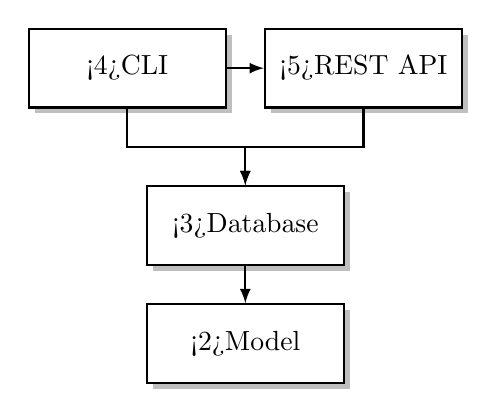
\begin{tikzpicture}[module/.style={minimum width=2.5cm,minimum height=1cm,draw,thick,drop shadow,fill=white},
                                dependency/.style={-latex,thick}]
                \node[module] (model) {\alert<2>{Model}};
                \node[module] (database) at ($ (model) + (0, 1.5) $) {\alert<3>{Database}};
                \node[module] (cli) at ($ (database) + (-1.5, 2) $) {\alert<4>{CLI}};
                \node[module] (rest) at ($ (database) + (1.5, 2) $) {\alert<5>{REST API}};

                \draw[dependency] (database) -- (model);
                \draw[dependency] (cli) -- ++(0,-1)  -| (database);
                \draw[dependency] (rest) -- ++(0,-1) -| (database);
                \draw[dependency] (cli) -- (rest);
            \end{tikzpicture}
        \end{column}
        \begin{column}{.5\textwidth}
            \begin{overprint}
                \onslide<2>
                \structure{Model}
                \begin{itemize}
                    \item Metadata tabellen
                    \item Types overeenkomstig domein
                        \begin{itemize}
                            \item Validatie
                            \item Formatting
                        \end{itemize}
                \end{itemize}

                \onslide<3>
                \structure{Database}
                \begin{itemize}
                    \item Squirrel voor opbouw SQL
                        \begin{itemize}
                            \item Tegen SQL injection
                        \end{itemize}
                    \item Modulaire query-functionaliteit
                        \begin{itemize}
                            \item Filtering
                            \item Paginering
                        \end{itemize}
                \end{itemize}

                \onslide<4>
                \structure{CLI}
                \begin{itemize}
                    \item Cobra library
                    \item Handig voor debuggen
                    \item Admin functionaliteit
                    \item Ondersteunt verbose mode
                    \item Configuratieopties
                \end{itemize}

                \onslide<5>
                \structure{REST API}
                \begin{itemize}
                    \item Gin library
                    \item E\'en endpoint (\texttt{/api/v1/documents})
                    \item Query parameters voor filters/paginering
                    \item Validatie
                \end{itemize}
            \end{overprint}
        \end{column}
    \end{columns}
\end{frame}

\begin{frame}
    \frametitle{Front-End Design}
    \begin{itemize}
        \item Component-based
        \item Inputvalidatie (niet te streng)
        \item Asynchronous requests
        \item Zod voor gevalideerde JSON
    \end{itemize}
\end{frame}

% \subsection{Verdere Ontwikkeling}
\frame{\tableofcontents[currentsubsection]}

\begin{frame}
    \frametitle{Mogelijke Verdere Ontwikkeling}
    \begin{itemize}
        \item Meer interactie met "klant"
            \begin{itemize}
                \item Huidige prototype "blind" ontwikkeld
            \end{itemize}
        \item Veiligheid
            \begin{itemize}
                \item HTTPS i.p.v.~HTTP
                \item Authenticatie m.b.v.~KUL systeem
            \end{itemize}
        \item Code
            \begin{itemize}
                \item Commentaar
                \item Tests
            \end{itemize}
        \item Systeembeheer
            \begin{itemize}
                \item Documentatie
                \item Configuratiebestand
            \end{itemize}
    \end{itemize}
\end{frame}

\begin{frame}
    \frametitle{Mogelijke Verdere Ontwikkeling}
    \begin{itemize}
        \item Database
            \begin{itemize}
                \item Gebruik echte database
                \item Meer queries
                \item Meer filters
                \item Sorteeropties
            \end{itemize}
        \item Gebruikersvriendelijkheid
            \begin{itemize}
                \item Autocomplete voor bedrijfsnummers
                \item Vriendelijkere documentnummer invoer
            \end{itemize}
        \item Betere gegevenspresentatie
            \begin{itemize}
                \item Duidelijkere tabel
                \item Downloadbaar (bv.~CSV, PDF)
            \end{itemize}
    \end{itemize}
\end{frame}


% \section{BCT Sales Website}
% % \frame{\tableofcontents[currentsection]}
% \subsection{Analyse}
\frame{\tableofcontents[currentsubsection]}

\begin{frame}
    \frametitle{Brussels Childbirth Trust}
    \begin{quotation}
        The Brussels Childbirth Trust is a volunteer-run, not-for-profit organisation that supports parents and families here in Belgium.
        We are the leading source of pregnancy, prenatal and parenting information in English.
        We are also a social and support community, helping you and your family to get out and about and meet other English-speaking families for playdates, learning and fun!
    \end{quotation}
    \begin{flushright}
        --- \href{https://bctbelgium.org/}{https://bctbelgium.org/}
    \end{flushright}
\end{frame}

\begin{frame}
    \frametitle{Verhaal}
    \structure{Probleemstelling}
    \begin{itemize}
        \item Kindjes groeien snel
        \item Duur om hun garderobe up to date te houden wegens constante ontgroeiing
    \end{itemize}

    \structure{Oplossing}
    \begin{itemize}
        \item \href{https://bct-sales.myaddr.io}{https://bct-sales.myaddr.io}
        \item Soort van Vinted
        \item Tweedehandskledij
        \item Leden stellen hun kinderkleding te koop via website
        \item Verkoopdag
            \begin{itemize}
                \item Alle artikels worden ingezameld op \'e\'en locatie
                \item Bezoekers kunnen artikels inspecteren en kopen
            \end{itemize}
    \end{itemize}
\end{frame}

\begin{frame}
    \frametitle{Organisatie: V\'o\'or de verkoopdag}
    \begin{itemize}
        \item \textit{Sellers} registreren hun artikels via website
        \item Elk artikel krijgt uniek nummer (ID) toegewezen
        \item Elk artikel krijgt een etiket
            \begin{itemize}
                \item Prijs
                \item ID
                \item Barcode-encodering van ID
                \item Beschrijving (antifraude)
            \end{itemize}
        \item Website genereert deze etiketten als PDF
    \end{itemize}
\end{frame}

\begin{frame}
    \frametitle{Organisatie: Op de verkoopdag}
    \begin{itemize}
        \item \textit{Cashiers} gebruiken website om verkopen te registreren
            \begin{itemize}
                \item Voeren IDs van gekochte artikels in
                \item Website toont prijs/beschrijving
                \item Cashier rondt artikelselectie af
                \item Website toont totaal
                \item Betaling wordt afgehandeld via Payconiq
                \item Cashier bevestigt verkoop
            \end{itemize}
        \item Barcodescanner voor snellere, minder foutgevoelige invoer IDs
        \item Website moet toelaten meermaals zelfde artikel te verkopen
        \item \textit{Admin} ziet verkoopcijfers in realtime
    \end{itemize}
\end{frame}

\begin{frame}
    \frametitle{Organisatie: Na de verkoopdag}
    \begin{itemize}
        \item \textit{Admin} vraagt verkochte artikels op
        \item Data uitvoeren naar CSV
        \item Admin stort verkoopsopbrengst naar \textit{sellers}
    \end{itemize}
\end{frame}

\begin{frame}
    \frametitle{Extra Vereisten}
    \begin{itemize}
        \item Installatie serversoftware zo eenvoudig mogelijk
        \item Bruikbaar vanop laptop/smartphone/tablet/\dots
        \item Gebruiksvriendelijke gebruikersinterface
            \begin{itemize}
                \item Validatie
                \item Eenvoudig
                \item Zelfdocumenterend (bv.~tooltips)
                \item Minimalistisch
            \end{itemize}
        \item Goedkope hosting
    \end{itemize}
\end{frame}

% \subsection{Architectuur}
\frame{\tableofcontents[currentsubsection]}

\begin{frame}
    \frametitle{Architectuur}
    \begin{center}
        \begin{tikzpicture}[label/.style={fill=blue!50,opacity=.9,minimum width=1.5cm,minimum height=0.5cm,font={\sc\tiny}},tech/.style={font=\tiny}]
            \begin{pgfonlayer}{foreground}
                \node[anchor=west] (server) { \includegraphics[width=1.5cm]{images/server.png} } node[anchor=north,tech] at (server.south) { \parbox{2cm}{\centering Go \\ Gin} };

                \node (seller) at ($ (server.west) + (-3,2.25) $) { \includegraphics[width=1cm]{images/computer.png} };
                % \node[anchor=north,tech] at (seller.south) { \parbox{2cm}{\centering TypeScript \\ React \\ Mantine} };
                \node[anchor=south,label] at (seller) { seller };

                \node (cashier) at ($ (server.west) + (-3,0) $) { \includegraphics[width=1cm]{images/computer.png} };
                % \node[anchor=north,tech] at (cashier.south) { \parbox{2cm}{\centering TypeScript \\ React \\ Mantine} };
                \node[anchor=south,label] at (cashier) { cashier };

                \node (admin) at ($ (server.west) + (-3,-2.25) $) { \includegraphics[width=1cm]{images/computer.png} };
                % \node[anchor=north,tech] at (admin.south) { \parbox{2cm}{\centering TypeScript \\ React \\ Mantine} };
                \node[anchor=south,label] at (admin) { admin };

                \node[anchor=west] (database) at ($ (server) + (3,0) $) { \includegraphics[width=1.5cm]{images/database.png} } node[anchor=north,tech] at (database.south) { SQLite3 };

                \draw[-latex,ultra thick] (seller) -- (server) node[midway,above,font=\tiny,sloped] { JSON };
                \draw[-latex,ultra thick] (cashier) -- (server) node[midway,above,font=\tiny,sloped] { JSON };
                \draw[-latex,ultra thick] (admin) -- (server) node[midway,above,font=\tiny,sloped] { JSON } node[midway,below,font=\tiny,sloped] { only readonly };
                \draw[-latex,ultra thick] let \p1=(admin), \p2=(server.south) in (admin) -- ($ (\x2,\y1) $) node[midway,above,font=\tiny] { CLI } node[midway,below,font=\tiny] { full functionality } -- ($ (server.south) + (0,-0.5) $);
                \draw[-latex,ultra thick] (server) -- (database) node[midway,above] { SQL };
            \end{pgfonlayer}

            \begin{pgfonlayer}{background}
                \draw[fill=black!50,opacity=.5] ($ (server.south west) + (-0.5,-0.6) $) rectangle ($ (database.north east) + (0.5,1) $);
                \node[anchor=north,black!75,font=\sc] at ($ (server.north west) ! .50 ! (database.north east) + (0,1) $) {aws lightsail server};
            \end{pgfonlayer}
        \end{tikzpicture}
    \end{center}

    \begin{tikzpicture}[overlay, remember picture]
        \node[anchor=south east,font=\tiny] at (current page.south east)  {
            images: Flaticon.com
        };
    \end{tikzpicture}
\end{frame}

\begin{frame}
    \frametitle{Motivering}
    \structure{Waarom \'e\'en server?}
    \begin{itemize}
        \item Eenvoud
        \item Lage kost
    \end{itemize}
    \vskip2mm
    \structure{Waarom LightSail?}
    \begin{itemize}
        \item Eenvoudig in gebruik
        \item Vaste maandelijkse kost
    \end{itemize}
    \vskip2mm
    \structure{Waarom SQLite3?}
    \begin{itemize}
        \item Wordt meegelinkt in Go executable
        \item Geen installatie/configuratie nodig
        \item In memory DB voor tests
        \item Volledige DB past in \'e\'en bestand
    \end{itemize}
\end{frame}

\begin{frame}
    \frametitle{Motivering}
    \structure{Waarom Go?}
    \begin{itemize}
        \item Statisch \& sterk getypeerd
        \item Lightweight
        \item Compilatie leidt tot \'e\'en executable zonder afhankelijkheden dankzij statically linked libraries
        \item Heeft nodige libraries (barcode generatie, PDF generatie, \dots)
    \end{itemize}
    \vskip2mm
    \structure{Waarom Admin CLI?}
    \begin{itemize}
        \item Oudere versies werkten zonder TLS
        \item Volledige adminfunctionaliteit enkel toegankelijk via SSH
            \begin{itemize}
                \item Gratis veiligheid
            \end{itemize}
        \item Sneller te implementeren als CLI dan webinterface
    \end{itemize}
\end{frame}

\begin{frame}
    \frametitle{Motivering}
    \structure{Waarom paswoorden in plaintext (heiligschennis)?}
    \begin{itemize}
        \item Veiligheid geen topprioriteit voor klant
        \item Potenti\"ele schade sowieso zeer beperkt
        \item Gebruikt om te beschermen tegen Murphy, niet Machiavelli
        \item Gemakkelijker voor organisatoren
    \end{itemize}
\end{frame}

% \subsection{Ontwerp}

% \subsubsection{DatabaseQuerier}
\frame{\tableofcontents[currentsubsection]}

\begin{frame}
    \frametitle{Probleemstelling}
    \begin{center}
        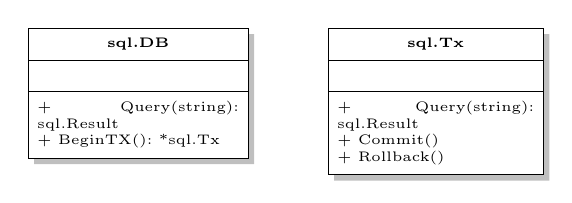
\begin{tikzpicture}[type/.style={minimum width=2cm,minimum height=1cm,fill=white,drop shadow,draw,rectangle split,rectangle split parts=3,font={\tiny}}]
            \node[type] (db) {
                \textbf{sql.DB}
                \nodepart{three}
                \parbox{2.56cm}{
                    + Query(string):\ sql.Result \\
                    + BeginTX():\ *sql.Tx
                }
            };

            \node[type,anchor=north west] (tx) at ($ (db.north east) + (1,0) $) {
                \textbf{sql.Tx}
                \nodepart{three}
                \parbox{2.5cm}{
                    + Query(string):\ sql.Result \\
                    + Commit() \\
                    + Rollback()
                }
            };
        \end{tikzpicture}
    \end{center}

    \begin{itemize}
        \item Go's \texttt{sql} library biedt twee types aan voor DB queries
            \begin{itemize}
                \item \texttt{sql.DB}
                \item \texttt{sql.Tx} voor transacties
            \end{itemize}
        \item Twee types queryfuncties
            \begin{itemize}
                \item Zij die zowel binnen als buiten transacties werken
                \item Zij die enkel binnen transacties werken
            \end{itemize}
        \item Transactie moeten uiteindelijk altijd oftewel \'e\'enmaal gecommit oftewel \'e\'enmaal gerollbackt worden
    \end{itemize}
\end{frame}

\begin{frame}
    \frametitle{Oplossing \#1: Interface Invoeren}
    \begin{center}
        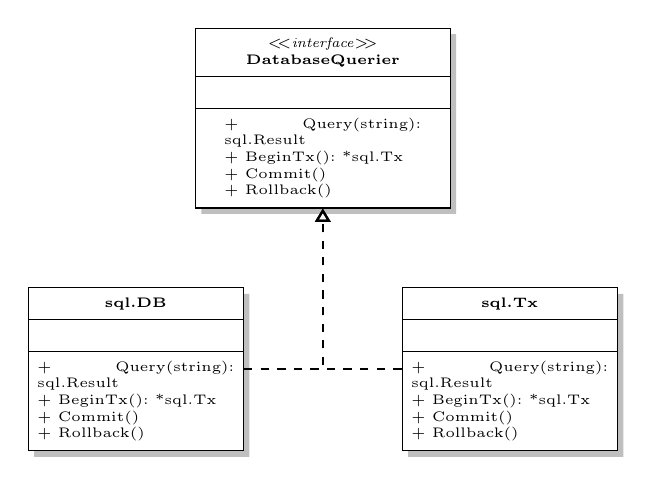
\begin{tikzpicture}[type/.style={minimum width=2cm,minimum height=1cm,fill=white,drop shadow,draw,rectangle split,font={\tiny}},
                            class/.style={type,rectangle split parts=3},
                            interface/.style={type,rectangle split parts=3}]
            \node[interface] (querier) {
                \parbox{3cm}{
                    \centering
                    \textit{\textless\!\!\textless interface\textgreater\!\!\textgreater}\\
                    \textbf{DatabaseQuerier}
                }
                \nodepart{three}
                \parbox{2.5cm}{
                    + Query(string):\ sql.Result \\
                    + BeginTx():\ *sql.Tx \\
                    + Commit() \\
                    + Rollback()
                }
            };

            \node[class,anchor=north east] (db) at ($ (querier.south) + (-1,-1) $) {
                \textbf{sql.DB}
                \nodepart{three}
                \parbox{2.5cm}{
                    + Query(string):\ sql.Result \\
                    + BeginTx():\ *sql.Tx \\
                    + Commit() \\
                    + Rollback()
                }
            };

            \node[class,anchor=west] (tx) at ($ (db.east) + (2,0) $) {
                \textbf{sql.Tx}
                \nodepart{three}
                \parbox{2.5cm}{
                    + Query(string):\ sql.Result \\
                    + BeginTx():\ *sql.Tx \\
                    + Commit() \\
                    + Rollback()
                }
            };

            \draw[-{Triangle[open]},thick,dashed] (db.east) -| (querier.south);
            \draw[-{Triangle[open]},thick,dashed] (tx.west) -| (querier.south);
        \end{tikzpicture}
    \end{center}
\end{frame}
\subsubsection{Observable Variables}
\frame{\tableofcontents[currentsubsection]}

\begin{frame}
    \frametitle{Probleemstelling}
    \begin{itemize}
        \item TUI
        \item Scheiding modellaag en presentatielaag
        \item Domein bevat data
        \item UI componenten krijgen elk klein stuk van domeindata te zien
    \end{itemize}
\end{frame}

\begin{frame}
    \frametitle{Design}
    \begin{center}
        \begin{tikzpicture}
            \draw[ultra thick] (0,0) -- (8,0);
            \node[anchor=south west] at (0,0) {Presentatie};
            \node[anchor=north west] at (0,0) {Domein};

            \node[anchor=north,font=\tiny,rectangle split,rectangle split parts=2,draw,inner sep=2pt] (item) at (4, -0.5) {
                \textbf{Item}
                \nodepart{two}
                \begin{tabular}{ll}
                    \textbf{Description} & "Blue shirt" \\
                    \textbf{Price} & 5 \\
                    \textbf{Category} & "Clothing 3-6 mos (56-62)" \\
                    \textbf{Donate} & true \\
                \end{tabular}
            };

            \node[anchor=south] at (4,0.2) { \includegraphics[height=3cm]{images/presentation.png} };
        \end{tikzpicture}
    \end{center}
\end{frame}

\begin{frame}
    \frametitle{Design}
    \begin{center}
        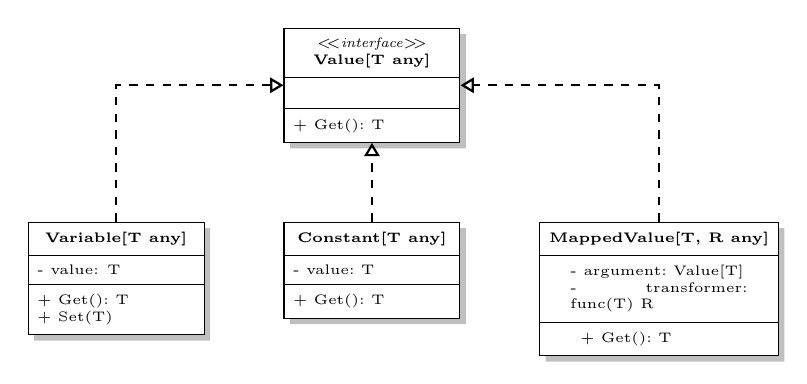
\begin{tikzpicture}[type/.style={minimum width=2cm,minimum height=1cm,fill=white,drop shadow,draw,rectangle split,font={\tiny}},
                            class/.style={type,rectangle split parts=3},
                            interface/.style={type,rectangle split parts=3}]
            \node[interface] (value) {
                \parbox{2cm}{
                    \centering
                    \textit{\textless\!\!\textless interface\textgreater\!\!\textgreater}\\
                    \textbf{Value[T any]}
                }
                \nodepart{three}
                \parbox{2cm}{
                    + Get():\ T
                }
            };

            \node[class,anchor=north east] (variable) at ($ (value.south west) + (-1,-1) $) {
                \textbf{Variable[T any]}
                \nodepart{two}
                \parbox{2cm}{
                    - value: T
                }
                \nodepart{three}
                \parbox{2cm}{
                    + Get():\ T \\
                    + Set(T)
                }
            };

            \node[class,anchor=north] (constant) at ($ (value.south) + (0,-1) $) {
                \textbf{Constant[T any]}
                \nodepart{two}
                \parbox{2cm}{
                    - value:\ T
                }
                \nodepart{three}
                \parbox{2cm}{
                    + Get():\ T
                }
            };

            \node[class,anchor=north west] (mappedvalue) at ($ (value.south east) + (1,-1) $) {
                \textbf{MappedValue[T, R any]}
                \nodepart{two}
                \parbox{2.25cm}{
                    - argument:\ Value[T] \\
                    - transformer:\ func(T) R
                }
                \nodepart{three}
                \parbox{2cm}{
                    + Get():\ T
                }
            };

            \draw[-{Triangle[open]},thick,dashed] (variable.north) |- (value.west);
            \draw[-{Triangle[open]},thick,dashed] (constant.north) -- (value.south);
            \draw[-{Triangle[open]},thick,dashed] (mappedvalue.north) |- (value.east);
        \end{tikzpicture}
    \end{center}
\end{frame}

\begin{frame}
    \frametitle{Design}
    \begin{center}
        \lstinputlisting[language=Go]{bct/valuemaps.go}
    \end{center}
\end{frame}

\begin{frame}
    \frametitle{Caching}
    \begin{itemize}
        \item Sommige transformaties zijn rekenintensief
        \item Caching
        \item Cache moet kunnen detecteren of herberekening nodig is
        \item Go biedt geen universele \texttt{equals} methode aan
        \item We werken daarom met versienummers
        \item Alternatief: elke value voorzien van een \texttt{func(T, T) bool}
    \end{itemize}
\end{frame}

\begin{frame}
    \frametitle{Design}
    \begin{center}
        \begin{tikzpicture}[type/.style={minimum width=2cm,minimum height=1cm,fill=white,drop shadow,draw,rectangle split,font={\tiny}},
                            class/.style={type,rectangle split parts=3},
                            interface/.style={type,rectangle split parts=3}]
            \node[interface] (value) {
                \parbox{2cm}{
                    \centering
                    \textit{\textless\!\!\textless interface\textgreater\!\!\textgreater}\\
                    \textbf{Value[T any]}
                }
                \nodepart{three}
                \parbox{2cm}{
                    + Get():\ T \\
                    \alert{+ Version():\ uint}
                }
            };

            \node[class,anchor=north east] (variable) at ($ (value.south west) + (-1,-1) $) {
                \textbf{Variable[T any]}
                \nodepart{two}
                \parbox{2cm}{
                    - value: T \\
                    \alert{- version: uint}
                }
                \nodepart{three}
                \parbox{2cm}{
                    + Get():\ T \\
                    + Set(T) \\
                    \alert{+ Version():\ uint}
                }
            };

            \node[class,anchor=north] (constant) at ($ (value.south) + (0,-1) $) {
                \textbf{Constant[T any]}
                \nodepart{two}
                \parbox{2cm}{
                    - value:\ T
                }
                \nodepart{three}
                \parbox{2cm}{
                    + Get():\ T \\
                    \alert{+ Version():\ uint}
                }
            };

            \node[class,anchor=north west] (cache) at ($ (value.south east) + (1,-1) $) {
                \textbf{Cache[T any]}
                \nodepart{two}
                \parbox{2.25cm}{
                    - value:\ Value[T] \\
                    - cached:\ T \\
                    - cachedVersion:\ uint
                }
                \nodepart{three}
                \parbox{2cm}{
                    + Get():\ T \\
                    + Version():\ uint
                }
            };

            \draw[-{Triangle[open]},thick,dashed] (variable.north) |- (value.west);
            \draw[-{Triangle[open]},thick,dashed] (constant.north) -- (value.south);
            \draw[-{Triangle[open]},thick,dashed] (mappedvalue.north) |- (value.east);
        \end{tikzpicture}
    \end{center}
\end{frame}

\begin{frame}
    \frametitle{Design}
    \begin{itemize}
        \item UI controls willen kunnen detecteren of waarde ge\"updatet werd sinds laatste rendering
        \item \texttt{View[T]} houdt bij welke versie laatst opgevraagd werd
    \end{itemize}
    \begin{center}
        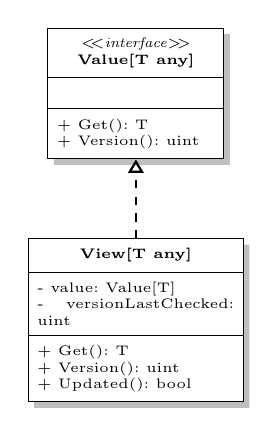
\begin{tikzpicture}[type/.style={minimum width=2cm,minimum height=1cm,fill=white,drop shadow,draw,rectangle split,font={\tiny}},
                            class/.style={type,rectangle split parts=3},
                            interface/.style={type,rectangle split parts=3}]
            \node[interface] (value) {
                \parbox{2cm}{
                    \centering
                    \textit{\textless\!\!\textless interface\textgreater\!\!\textgreater}\\
                    \textbf{Value[T any]}
                }
                \nodepart{three}
                \parbox{2cm}{
                    + Get():\ T \\
                    \alert{+ Version():\ uint}
                }
            };

            \node[class,anchor=north] (view) at ($ (value.south) + (0,-1) $) {
                \textbf{View[T any]}
                \nodepart{two}
                \parbox{2.5cm}{
                    - value:\ Value[T] \\
                    - versionLastChecked:\ uint
                }
                \nodepart{three}
                \parbox{2.5cm}{
                    + Get():\ T \\
                    + Version():\ uint \\
                    + Updated():\ bool
                }
            };

            \draw[-{Triangle[open]},thick,dashed] (view.north) -- (value.south);
        \end{tikzpicture}
    \end{center}
\end{frame}

\begin{frame}
    \frametitle{Design}
    \lstinputlisting[language=Go]{bct/valueexample.go}
\end{frame}

\begin{frame}
    \frametitle{Design}
    \begin{itemize}
        \item Oorspronkelijk werkte TUI met observeerbare variabelen
        \item Observers kregen echter inconsistente data te zien
        \item Manier nodig om observer-updates te groeperen
        \item Laziness werd hiervoor ingevoerd
    \end{itemize}
\end{frame}

\subsubsection{RestStatus}
\frame{\tableofcontents[currentsubsection]}

\begin{frame}
    \frametitle{RestStatus}
    \structure{Probleemstelling}
    \begin{itemize}
        \item In front-end code (TypeScript)
        \item Asychrone request heeft drie toestanden
    \end{itemize}
    \vskip2mm
    \begin{overprint}
        \onslide<1>
        \begin{center}
            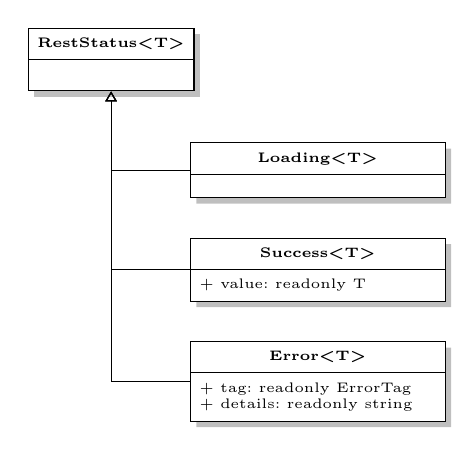
\begin{tikzpicture}[type/.style={minimum width=2cm,minimum height=1cm,fill=white,drop shadow,draw,rectangle split,rectangle split parts=2,font={\tiny}}]
                \node[type] (reststatus) {\textbf{RestStatus\textless T\textgreater}};

                \node[anchor=west,type] (loading) at ($ (reststatus.south) + (1,-1) $) {
                    \textbf{Loading\textless T\textgreater}
                    \nodepart{two}
                    \parbox{3cm}{\ }
                };

                \node[anchor=north west,type] (success) at ($ (loading.south west) + (0,-0.5) $) {
                    \textbf{Success\textless T\textgreater}
                    \nodepart{two}
                    \parbox{3cm}{
                        + value:\ readonly T
                    }
                };

                \node[anchor=north west,type] (error) at ($ (success.south west) + (0,-0.5) $) {
                    \textbf{Error\textless T\textgreater}
                    \nodepart{two}
                    \parbox{3cm}{
                        + tag:\ readonly ErrorTag \\
                        + details:\ readonly string
                    }
                };

                \draw[-{Triangle[open]}] (loading) -| (reststatus);
                \draw[-{Triangle[open]}] (success) -| (reststatus);
                \draw[-{Triangle[open]}] (error) -| (reststatus);
            \end{tikzpicture}
        \end{center}

        \onslide<2>
        \lstinputlisting[language=TypeScript]{bct/reststatus-classes.ts}

    \end{overprint}
\end{frame}

\begin{frame}
    \frametitle{Probleemstelling}
    \begin{itemize}
        \item Toestandsafhankelijke code
            \begin{itemize}
                \item Toestand bepaalt welke UI component getoond wordt
            \end{itemize}
        \item Exhaustiviteitscheck
            \begin{itemize}
                \item Elke toestand moet expliciet afgehandeld worden
                \item Zoniet compilerfout
            \end{itemize}
    \end{itemize}
\end{frame}

\begin{frame}
    \frametitle{Poging \#1: Switch op Type}
    \lstinputlisting[language=TypeScript]{bct/instanceof.ts}
    \begin{itemize}
        \item Fragiel
        \item Ontbrekende gevallen niet gedetecteerd
    \end{itemize}
\end{frame}

\begin{frame}
    \frametitle{Poging \#2: Visitor Design Pattern}
    \lstinputlisting[language=TypeScript]{bct/visitor.ts}
    \begin{itemize}
        \item Robuust, maar zeer omslachtig
    \end{itemize}
\end{frame}

\begin{frame}
    \frametitle{Poging \#3: Discriminated Unions}
    \lstinputlisting[language=TypeScript]{bct/discrimated-union.ts}
    \begin{itemize}
        \item Combinatie singleton types en union types
        \item Robuust
        \item Lichte syntax
    \end{itemize}
\end{frame}


\section{Fin}
\frame{\tableofcontents[currentsection]}
\begin{frame}
    \frametitle{Gekende Programmeertalen}
    \begin{columns}[t]
        \begin{column}{.45\textwidth}
            \begin{center}
                \begin{tabular}{ll}
                    \toprule
                    \multicolumn{2}{c}{\textbf{Industrie}} \\
                    \midrule
                    Python & \rating{5} \\
                    Ruby & \rating{5} \\
                    Java & \rating{5} \\
                    JavaScript & \rating{5} \\
                    TypeScript & \rating{5} \\
                    Go & \rating{5} \\
                    \csharp & \rating{5} \\
                    \cpp & \rating{4} \\
                    C & \rating{3} \\
                    Rust & \rating{3} \\
                    Elixir & \rating{2} \\
                    \bottomrule
                \end{tabular}
            \end{center}
        \end{column}
        \begin{column}{.45\textwidth}
            \begin{center}
                \begin{tabular}{ll}
                    \toprule
                    \multicolumn{2}{c}{\textbf{Academisch}} \\
                    \midrule
                    O'Caml & \rating{5} \\
                    \LaTeX & \rating{5} \\
                    Common Lisp & \rating{4} \\
                    Racket & \rating{4} \\
                    Haskell & \rating{4} \\
                    Wolfram Language & \rating{4} \\
                    Coq & \rating{4} \\
                    Prolog & \rating{3} \\
                    Oz & \rating{2} \\
                    Maude & \rating{1} \\
                    \bottomrule
                \end{tabular}
            \end{center}
        \end{column}
    \end{columns}
\end{frame}

\begin{frame}
    \frametitle{Gebruikte Frameworks}
    \begin{center}
        \begin{tabular}{ll}
            \toprule
            \textbf{Framework} & \textbf{Taal} \\
            \midrule
            Sinatra & Ruby \\
            Flask & Python \\
            FastAPI & Python \\
            Gin & Go \\
            Bubble Tea & Go \\
            tview & Go \\
            WPF & \csharp \\
            Swing & Java \\
            React & TypeScript \\
            \bottomrule
        \end{tabular}
    \end{center}
\end{frame}

\end{document}
